\documentclass[twocolumn,a4j]{jsarticle}
\bibliographystyle{junsrt}

\setlength{\topmargin}{-20.4cm}
\setlength{\oddsidemargin}{-10.4mm}
\setlength{\evensidemargin}{-10.4mm}
\setlength{\textwidth}{18cm}
\setlength{\textheight}{26cm}

\usepackage[top=15truemm,bottom=20truemm,left=20truemm,right=20truemm]{geometry}
\usepackage[latin1]{inputenc}
\usepackage{amsmath}
\usepackage{amsfonts}
\usepackage{amssymb}
\usepackage[dvipdfmx]{graphicx}
\usepackage[hang,small,bf]{caption}
\usepackage[subrefformat=parens]{subcaption}
\usepackage[dvipdfmx]{color}
\usepackage{listings}
\usepackage{listings,jvlisting}
\usepackage{geometry}
\usepackage{framed}
\usepackage{color}
\usepackage[dvipdfmx]{hyperref}
\usepackage{ascmac}
\usepackage{enumerate}
\usepackage{tabularx}
\usepackage{cancel}
\usepackage{scalefnt}
\usepackage{overcite}
\usepackage{otf}

\renewcommand{\figurename}{Fig.}
\renewcommand{\tablename}{Table }

\hypersetup{%
    hidelinks %リンクの色消し
}

\lstset{
basicstyle={\ttfamily},
identifierstyle={\small},
commentstyle={\smallitshape},
keywordstyle={\small\bfseries},
ndkeywordstyle={\small},
stringstyle={\small\ttfamily},
frame={tb},
breaklines=true,
columns=[l]{fullflexible},
xrightmargin=0zw,
xleftmargin=3zw,
numberstyle={\scriptsize},
stepnumber=1,
numbersep=1zw,
lineskip=-0.5ex
}

% キャプション後ろのダブルコロンを消す
\makeatletter
\long\def\@makecaption#1#2{%
  \vskip\abovecaptionskip
  \iftdir\sbox\@tempboxa{#1\hskip1zw#2}%
    \else\sbox\@tempboxa{#1 #2}%
  \fi
  \ifdim \wd\@tempboxa >\hsize
    \iftdir #1\hskip1zw#2\relax\par
      \else #1 #2\relax\par\fi
  \else
    \global \@minipagefalse
    \hbox to\hsize{\hfil\box\@tempboxa\hfil}%
  \fi
  \vskip\belowcaptionskip}
\makeatother


\makeatletter
\def\@maketitle
{
\begin{center}
{\LARGE \@title \par}
\end{center}
\begin{flushright}
{\large \@date}\\
{\large 京都工芸繊維大学 大学院 機械設計学専攻 計測システム工学研究室}\\
{\large M2 \@author}
\end{flushright}
\par\vskip 1.5em
}
\makeatother

\author{来代 勝胤 / KITADAI Masatsugu}
\title{令和5年度 5月度 共同研究 報告書}
\date{2023/05/23}

\begin{document}
\columnseprule=0.1mm
\maketitle

\section*{報告内容}
\begin{enumerate}[1.]
  \item 数値シミュレーションによる計測手法の評価
  \item 三角翼後流の計測
  \item 車両モデル周りの流れ計測
  \item 6月の予定
\end{enumerate}

\section*{進捗報告}
今月は,ISTPへの投稿に向けた数値シミュレーションデータの作成と解析および
可視化情報シンポジウムの原稿作成に向けた
三角翼後流と車両モデル周りにおける二次流れの計測実験を行った.

\section{数値シミュレーションによる計測手法評価}
\subsection{作成する数値シミュレーションの条件}
先月に引き続き,数値シミュレーションを用いた
計測アルゴリズム評価に向け,以下に示す解析解について
Table.1 に示す条件に沿ってデータを作成した.
また,粒子数密度及び壁面の回転速度を Table.2 のように
変更し,合計9つのパターンについて計算を行った.\\

\subsection*{流れの解析解}
\begin{eqnarray*}
  \zeta &=& z \sqrt{\frac{\omega}{\nu}}\\
  V_r &=& r \omega F \left(\zeta\right)\\
  V_\theta &=& r \omega G \left(\zeta\right)\\
  u &=& \sqrt{\nu \omega} H \left(\zeta\right)
\end{eqnarray*}

\begin{table}[hbtp]
  \label{table:data_type}
  \caption{シミュレーション条件}
  \centering
  \begin{tabular}{ c c | r l}
    \hline
    動粘性係数              & $\nu$        & $1.004 \times 10^{-6}$ & [$\mathrm{m}^2$/s] \\ \hline
    $\mathrm{LLS}_1$ の位置 & $x_0$        & 7.000                  & [mm]               \\ \hline
    $\mathrm{LLS}_1$ の厚み & $T_1$        & $3.086\times 10^{-3}$  & [mm]               \\ \hline
    $\mathrm{LLS}_2$ の厚み & $T_2$        & $9.259\times 10^{-3}$  & [mm/s]             \\ \hline
    LLS 間の距離            & $\Delta x$   & $9.645\times 10^{-3}$  & [mm/s]             \\ \hline
    撮影範囲                & $y \times z$ & $40 \times 40$         & [mm]               \\ \hline
    画像サイズ              & $w \times h$ & $800 \times 800$       & [px]               \\ \hline
  \end{tabular}
\end{table}

\begin{table}[hbtp]
  \label{table:data_type}
  \caption{数値シミュレーション条件}
  \centering
  \begin{tabular}{c c c}
    \hline
           & \textgt{粒子数密度} [-/枚] & \textgt{角速度} [deg/s] \\ \hline \hline
    Case 1 & 100                        & 10.0                    \\ \hline
    Case 2 & 200                        & 10.0                    \\ \hline
    Case 3 & 300                        & 10.0                    \\ \hline
    Case 4 & 100                        & 5.0                     \\ \hline
    Case 5 & 200                        & 5.0                     \\ \hline
    Case 6 & 300                        & 5.0                     \\ \hline
    Case 7 & 100                        & 15.0                    \\ \hline
    Case 8 & 200                        & 15.0                    \\ \hline
    Case 9 & 300                        & 15.0                    \\ \hline
  \end{tabular}
\end{table}

\newpage
\subsection{速度場の真値とPIV結果}

Fig.1 に Case 1 における速度場の真値,
Fig.2 に Case 1 の数値シミュレーションにPTVを適用した結果を示す.
FIg.2 にはベクトルの抜けはあるが回転の方向と速度の大きさが
一致していることが確認できる.

\begin{table}[hbtp]
  \label{table:data_type}
  \caption{RMSEによる誤差の値と誤差率}
  \centering
  \begin{tabular}{ c c c }
    \hline
           & Error ratio of RMSE [\%] \\ \hline \hline
    Case 1 & 5.654                    \\ \hline
    Case 2 & 5.915                    \\ \hline
    Case 3 & 7.220                    \\ \hline
  \end{tabular}
\end{table}

また Table.3 にCase.1 ~ Case.3 についてRMSE率を示している.
結果を見ると粒子数密度が上がるにつれて
真値との差が広がっていることが確認でき,
Case 2 と Case 3 の間に計測精度が大きく低下することがわかる.

\newpage

\begin{figure}[htbp]
  \footnotesize
  \begin{center}
    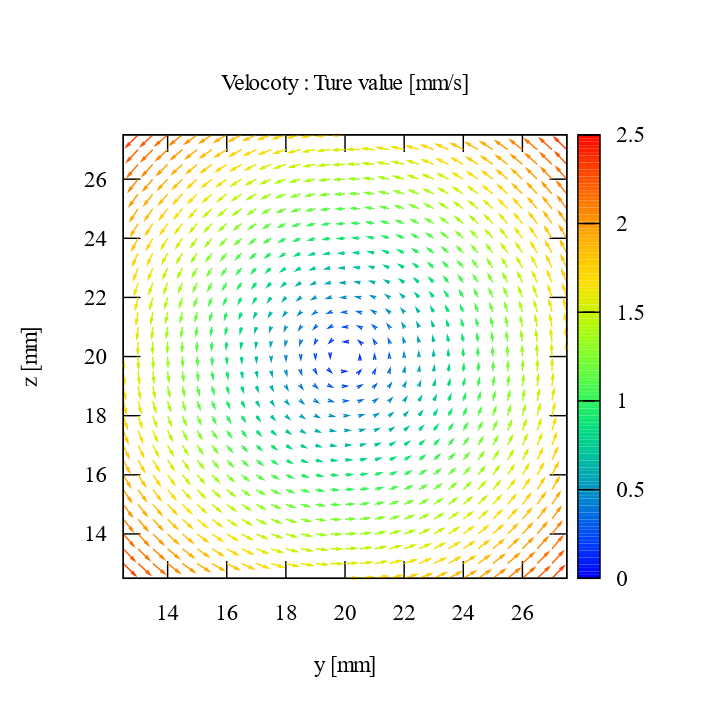
\includegraphics[width=80mm]{../images/vector_true_value.png}
    \caption{True value of velocity : Case 1}
    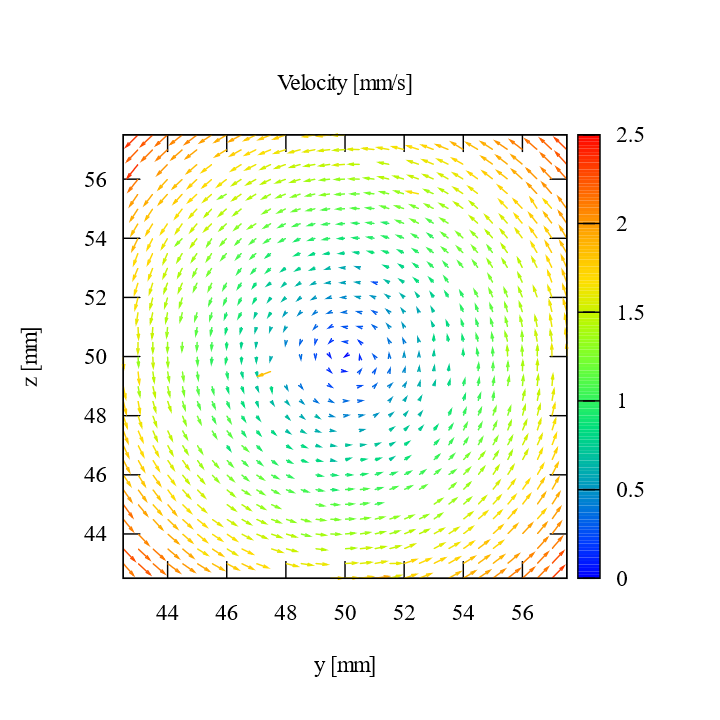
\includegraphics[width=80mm]{../images/vector_simulation.png}
    \caption{PIV result of velocity : Case 1}
  \end{center}
\end{figure}

\section{三角翼後流の計測}
可視化情報シンポジウムの原稿作成に向けて
三角翼後流の流れ場の撮影を再度行った.\\

\subsection{計測位置について}
今回は,Fig.3に示す三角翼モデルの後流について
Fig.4のように設置し,後方50mmの位置を対象として計測を行った.
また,撮影条件は以下の Table 4 の通りである.

\begin{table}[h]
  \label{table:data_type}
  \centering
  \caption{Experimental conditions}
  \begin{tabular}{| l | r | l |}
    \hline
    Mainstream velocity   & 250              & [mm/s]  \\ \hline
    Laser sheets distance & 2.5              & [mm]    \\ \hline
    Image size            & 800 $\times$ 600 & [px]    \\ \hline
    Frame rate            & 800              & [fps]   \\ \hline
    Shutter Speed         & 1/1000           & [s]     \\ \hline
    number of shots       & 4000             & [sheet] \\ \hline
  \end{tabular}
\end{table}

\begin{figure}[htbp]
  \footnotesize
  \begin{center}
    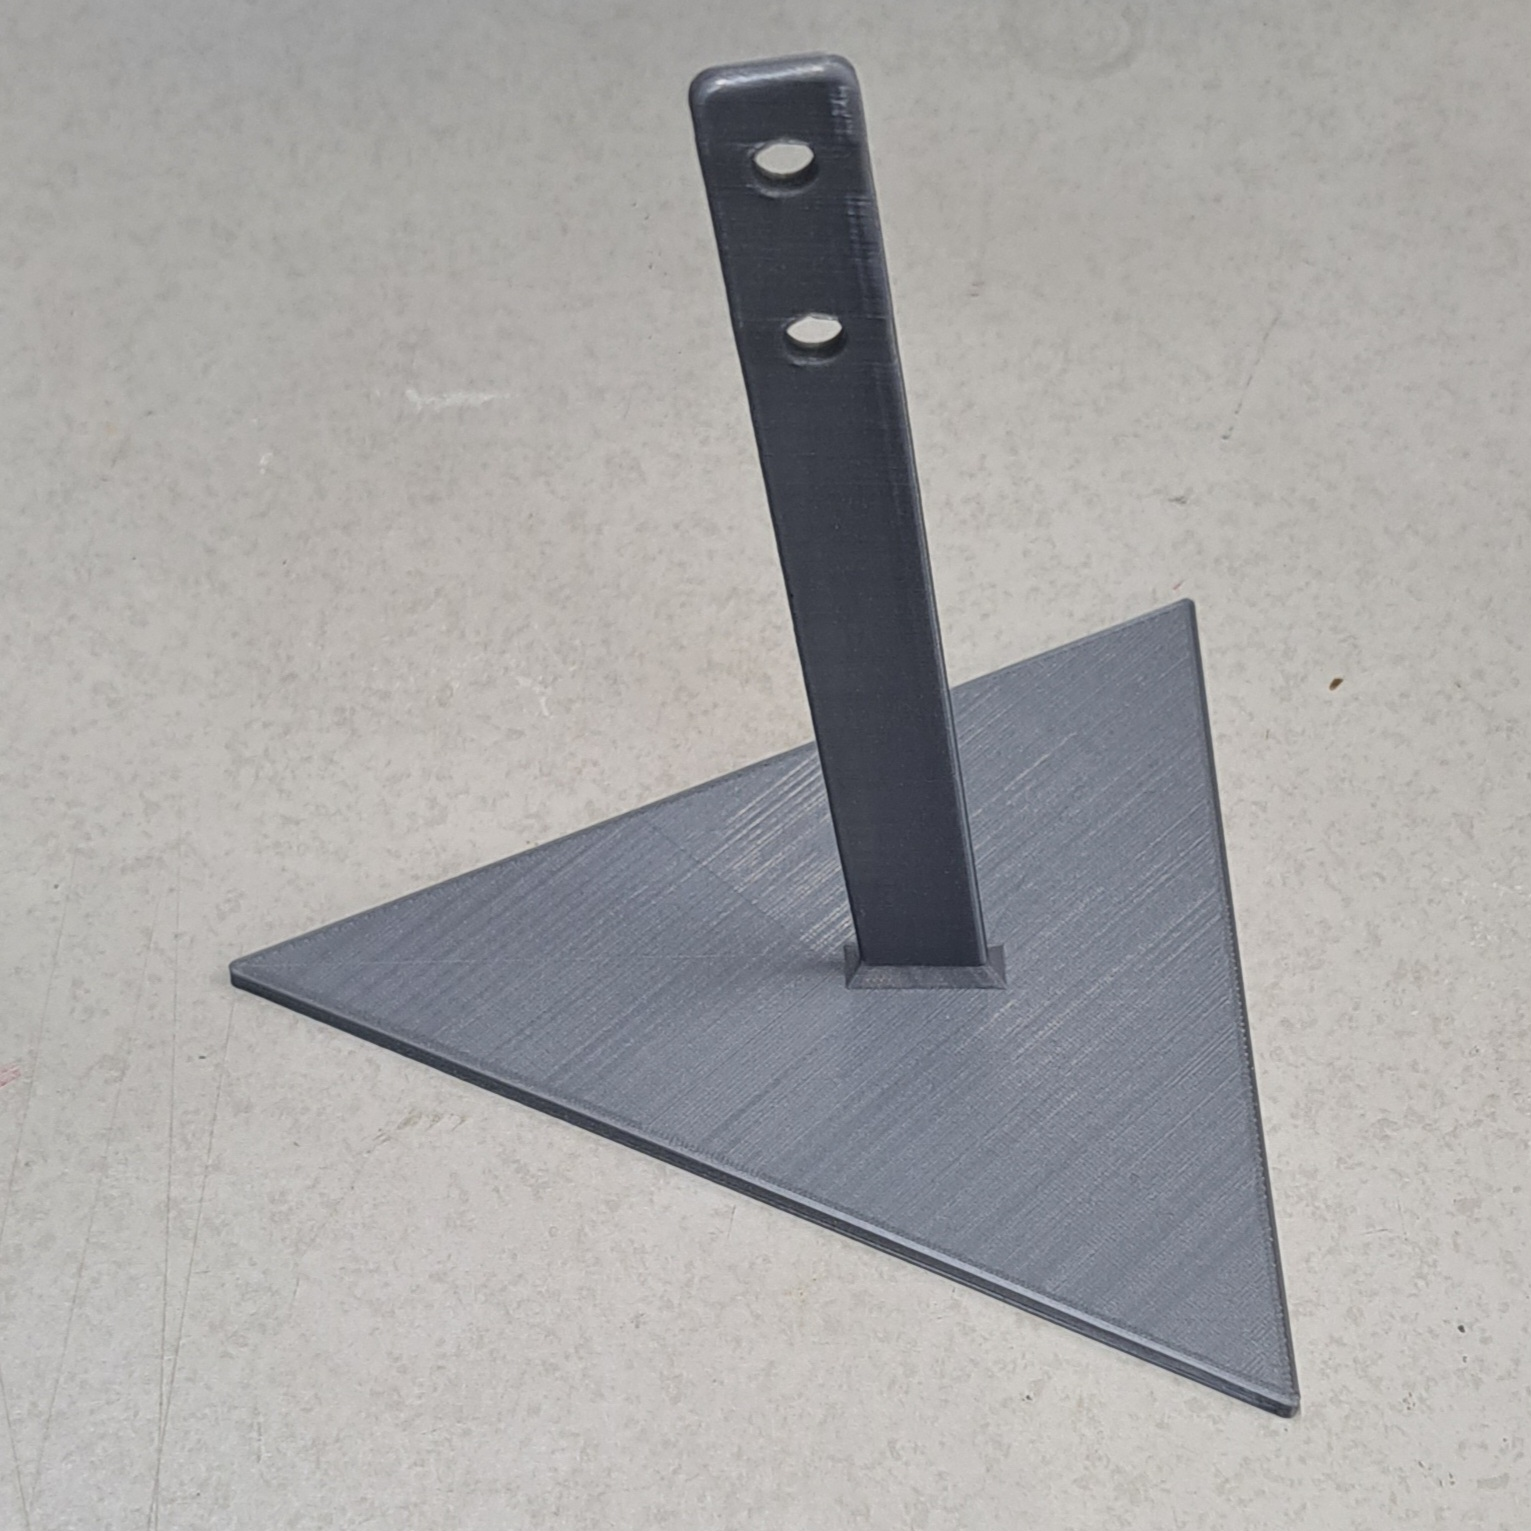
\includegraphics[width=50mm]{../images/delta_wing_model.jpg}
    \caption{Delta wing model}
    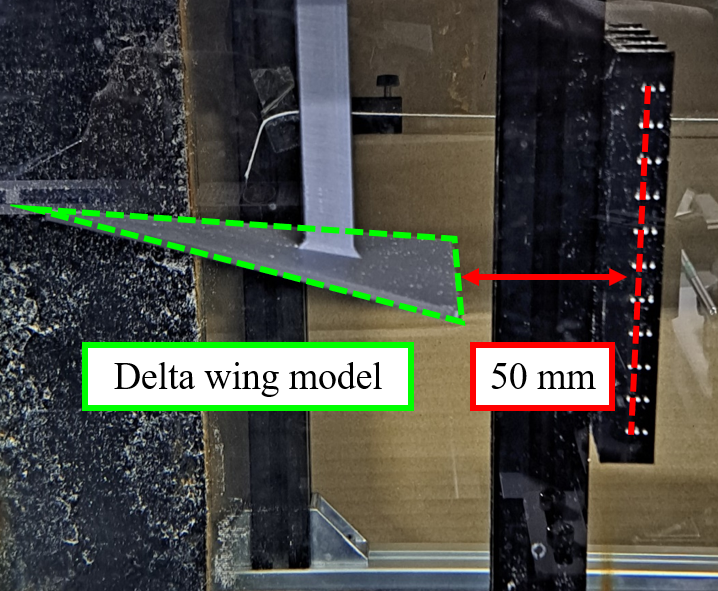
\includegraphics[width=60mm]{../images/delta_wing_position.png}
    \caption{Measurement position of delta wing wake}
  \end{center}
\end{figure}

\newpage

\subsection{解析結果}
Fig.5 にPTVの時間平均結果を示す.
結果より,$(y,z) = (50, 15)$を中心として反時計回りの渦の発生を見ることができる.
一方で渦の左側が鮮明に解析されていることに対して,右側は形が崩れていることもわかる.
これは,斜め後方からの撮影によって,カメラ手前側に当たる左側の情報量が大きく
奥側に当たる右側の情報量が少ない影響であると考える.

\begin{figure}[htbp]
  \footnotesize
  \begin{center}
    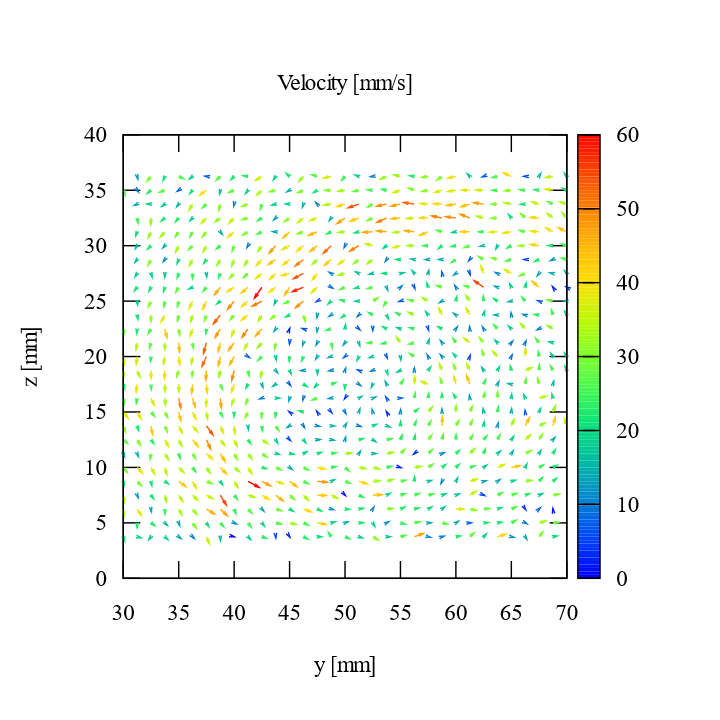
\includegraphics[width=80mm]{../images/delta_wing.png}
    \caption{Time-averaged velocity for wake of delta}
  \end{center}
\end{figure}

\newpage

\section{車両モデル周りの流れ計測}

\subsection{車両モデルの設置}
続いて,車両モデルを用いた流れの計測を行うにあたり,
回流水槽にFig.6 に示すようにタイヤモデル及び車体モデルを取り付け
設置した.また,タイヤモデルは主流速度に対応して回転させることができる.
一方,地面板については以前使用していたものを使用しているため,
再度撥水加工を行う予定である.

\begin{figure}[htbp]
  \footnotesize
  \begin{center}
    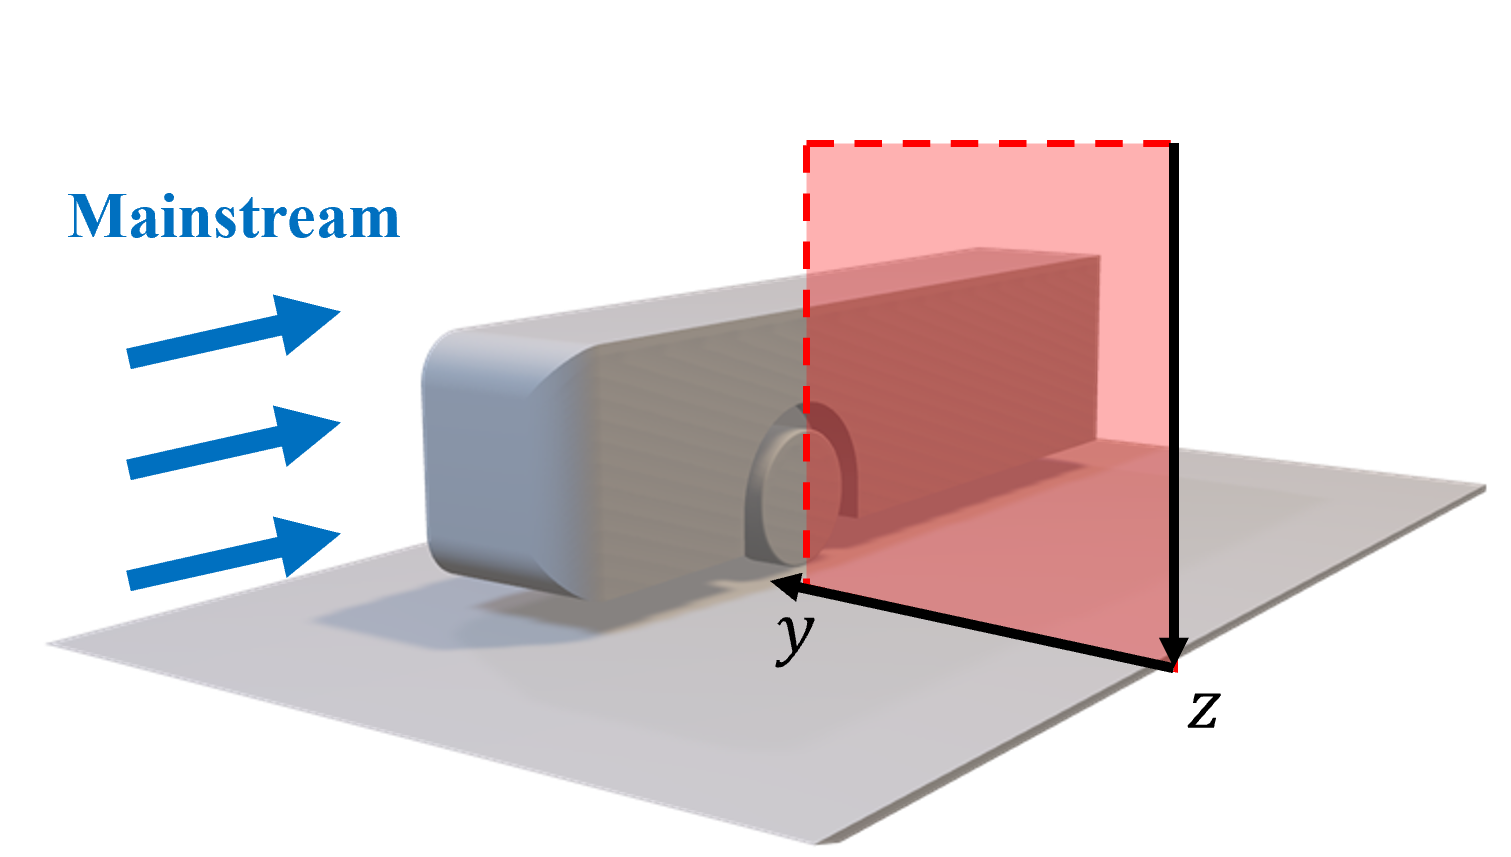
\includegraphics[width=60mm]{../images/vehicle_model.png}
    \caption{Vehicle model}
  \end{center}
\end{figure}

\subsection*{計測位置について}
今回の計測は,Fig.7に示すようにLLSを設置し,
車両モデルのタイヤ車軸から後方50mmの位置を撮影した.
なお,撮影は三角翼後流と同様に
Table 4 に示す条件で行った.

\begin{figure}[htbp]
  \footnotesize
  \begin{center}
    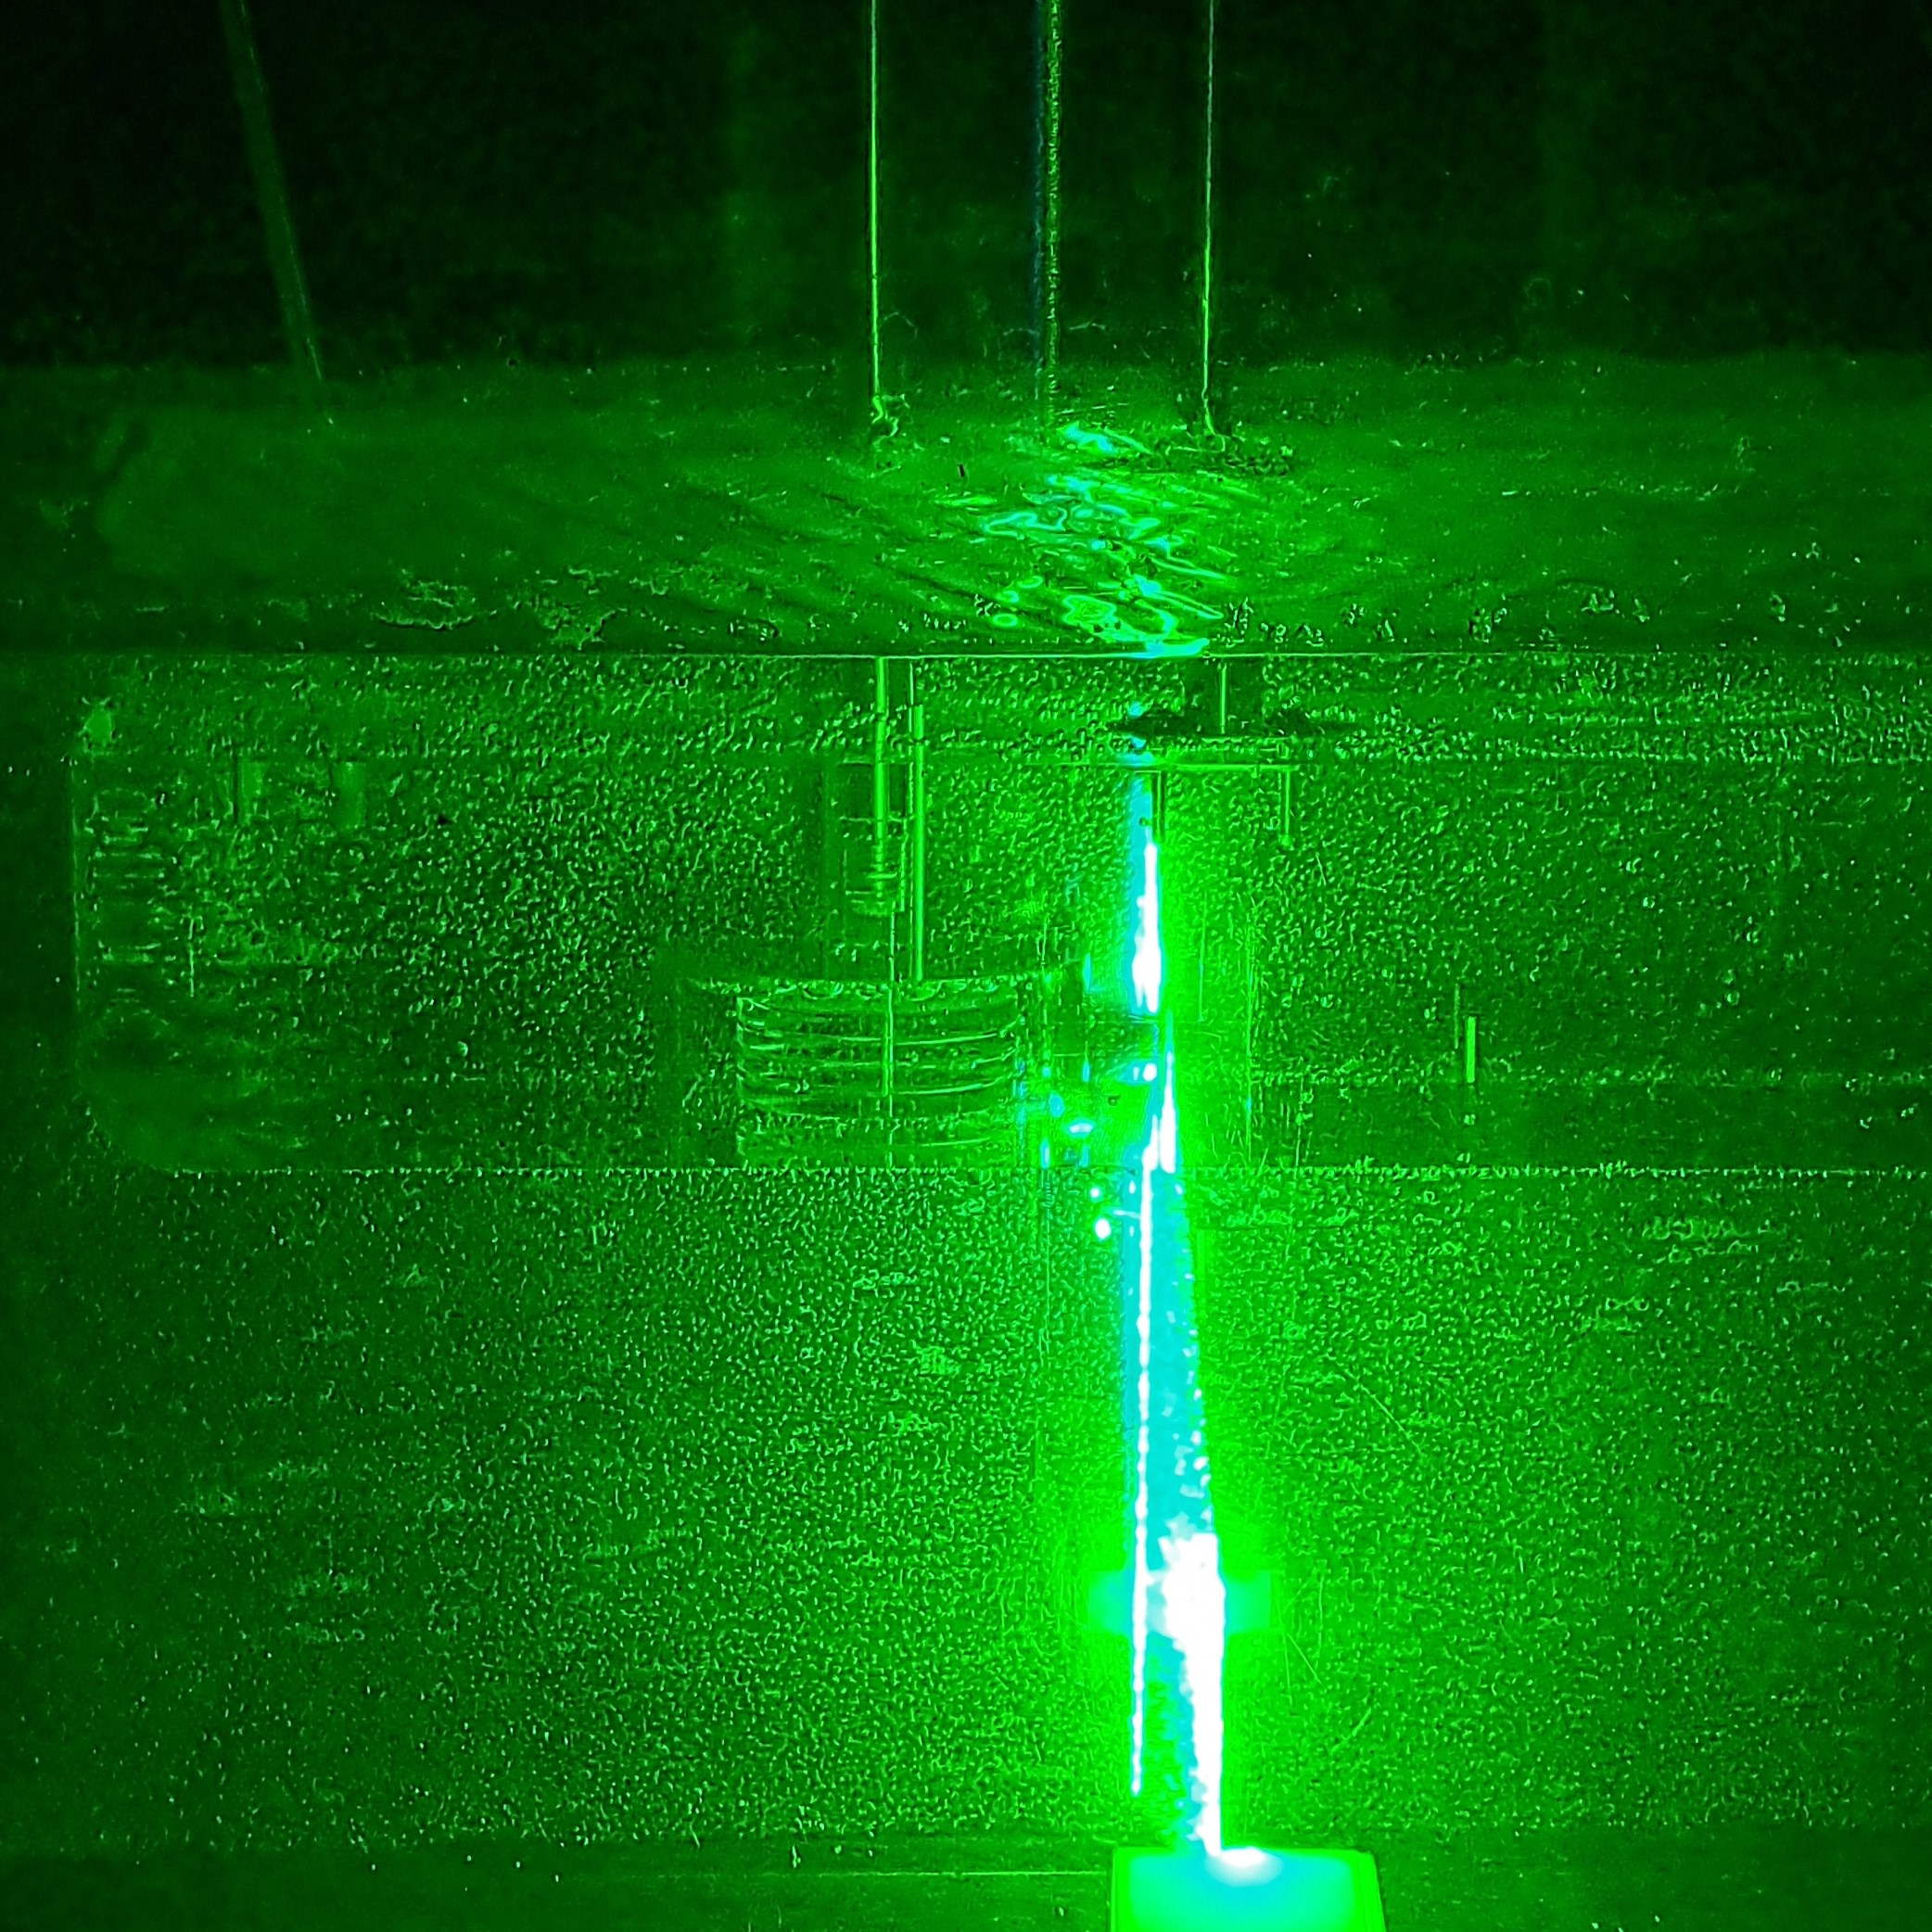
\includegraphics[width=50mm]{../images/experiment.jpg}
    \caption{Measurement position of wheelhouse wake}
  \end{center}
\end{figure}

\newpage
\subsection*{解析結果}
Fig.8にPTVの時間平均結果を示す.
結果の上部にタイヤモデルが設置されているためベクトルの表示はない.
結果をみると,三角翼のように定常的な流れの発生ではないことから
時間平均の流れ場に定常性はないことが確認できる.
車両モデルの二次流れの撮影は達成したが,
データの解析方法及び撮影条件については今後検討する必要がある.

\begin{figure}[htbp]
  \footnotesize
  \begin{center}
    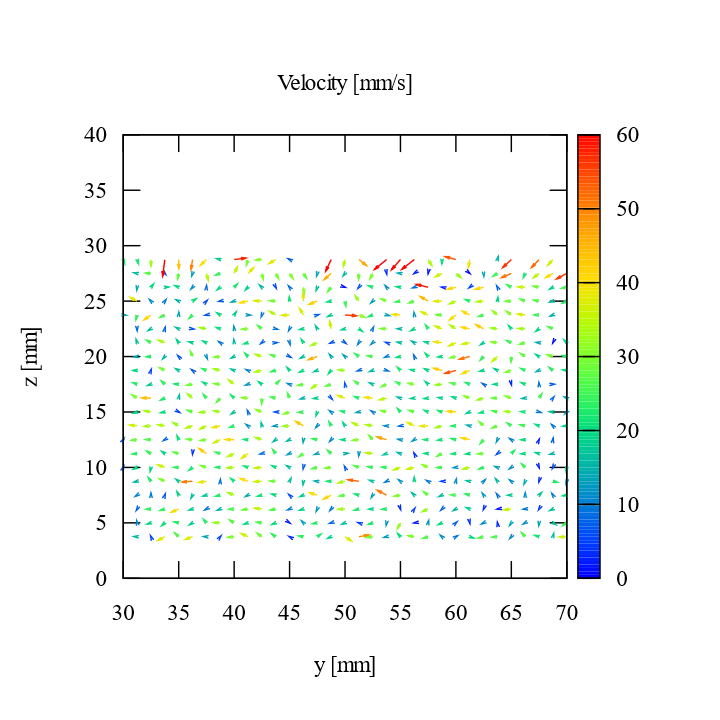
\includegraphics[width=80mm]{../images/tyre.png}
    \caption{Time-averaged velocity for wake of wheelhouse}
  \end{center}
\end{figure}

\section{6月の予定}
\begin{itemize}
  \item 可視化情報シンポジウム 原稿提出 (5/31)
  \item 数値シミュレーションの結果整理
  \item ISTP 原稿提出 (6/30)
\end{itemize}


\end{document}